\javalstset{}{}
\FloatBarrier
\subsubsection{Die Bibliothek \emph{gdata}}
Die Google-Bibliothek \emph{gdata} ist eine frei verf\"ugbare Bibliothek zum erstellen von
 Clientapplications für die Services der Google-Cloud.
\emph{gdata} kapselt die Webservices komplett in Java-Klassen, so dass ein importieren
 (z.\ B.\ mit \wsimport) nicht mehr notwendig ist.

In der Beschreibung der \emph{gdata}-Bibliothek wird beschrieben, wie man aus der zip-Datei
 ein JAR compilieren kann, da dies bei mir in mehreren Versuchen nicht geklappt hat,
 haben wir die pragmatische Lösung gewählt und die in der zip-Datei enthaltenen JARs einzeln
 in das Projekt eingefügt\cite{GO02}.
\FloatBarrier
\subsubsection{Authentifizieren und Verbinden mit \emph{gdata}}
Google bietet zwei Authentifizierungsverfahren an
\begin{enumerate}
	\item\emph{OAuth}
	\item Username und Passwort
\end{enumerate}
\emph{OAuth} ist ein Service, der bei erfolgreicher Anmeldung ein Token erstellt, mit dem
 der Client von Google bereitgestellte Services aufrufen und sich authentifizieren kann.
So muss der Client die Anmelde-Daten des Nutzers nicht speichern, sondern nur den Token.
In Abbildung \ref{fig:google_oauth} wird ein Beispiel f\"ur die Nutzung von \emph{OAuth}
 dargestellt.
\begin{figure}[h!]
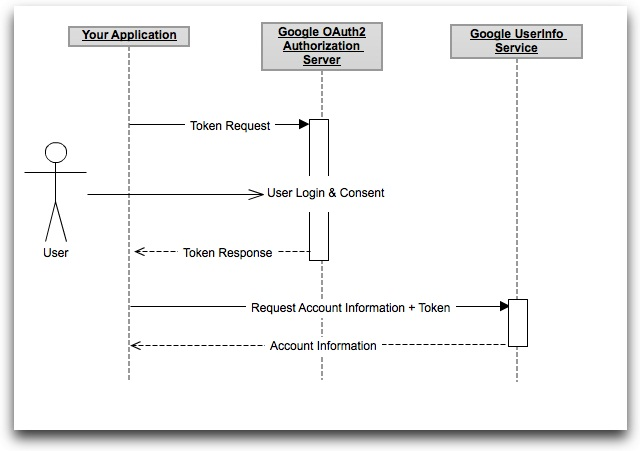
\includegraphics[width=\textwidth]{Bilder/googleOauth.jpg}
\caption{Nutzungsbeispiel f\"ur \emph{OAuth}\cite{GO01}}
\label{fig:google_oauth}
\end{figure}

Da wir unseren eigenen Account nutzen und die Daten nicht sicherheitskritisch sind, haben
 wir die zweite Variante gew\"ahlt und authentifizieren uns bei jedem Service-Aufruf mit
 Username und Passwort.

Die Authentifizierung wird für ein \lstinline{ContacsService}-Objekt, wie in Listing
 \ref{lst:authpwbeispiel} abgebildet, einmal durchgeführt, danach wird sie vom Framework
 automatisch durchgeführt.
 \\
In der Abbildung wird ein \lstinline{ContactsService}-Objekt erstellt.
Der \lstinline{String}-Parameter \lstinline{servicename} dient hier als Identifikator für den Nutzer.
\\
Nachdem das \lstinline{ContactsService}-Objekt erstellt ist, wird der Service mit Nutzername und
 Passwort angemeldet.
 
\javalstset{Beispiel für die Authentifizierung ohne \emph{OAuth}}{lst:authpwbeispiel}
\begin{lstlisting}[float=h!t]
ContactsService myService;
myService = new ContactsService(servicename);
try {
	myService.setUserCredentials(username, password);
} catch (AuthenticationException e) {
	e.printStackTrace();
}
\end{lstlisting}

\FloatBarrier
\subsubsection{Kontakte suchen}
Die \emph{gdata}-Bibliothek bietet die Möglichkeit, Kontakte wie in Listing \ref{lst:searchQuery}
 mit Angabe eines \lstinline{Query}-Objekts herunterzuladen.
Im Codebeispiel wird das \lstinline{Query}-Objekt \lstinline{myQuery} für die hinter der URL
 \lstinline{feedURL} liegenden Kontakte initialisiert, danach wird es durch die
 \lstinline{"group"}-Option angewiesen nur Kontakte aus der Gruppe mit dem
 \lstinline{String}-Identifikator \lstinline{groupId} herunterzuladen.
Nachdem \lstinline{myQuery} konfiguriert ist, wird mit dem authentifizierten
 \lstinline{ContactsService} \lstinline{myService} der Service-Aufruf per
 \lstinline{query()}-Befehl ausgeführt.
Die Klasse \lstinline{Query} kann allerdings nur zwischen Gruppen unterscheiden, jedoch nicht nach
 anderen Kriterien wie z.\ B.\ dem Vornamen oder dem Nachnamen eines Kontakts filtern.

\javalstset{Kontaktsuche per \lstinline{Query}}{lst:searchQuery}
\begin{lstlisting}[float=h!t]
URL feedUrl = new URL(contactsURL);
Query myQuery = new Query(feedUrl);
ContactFeed resultFeed = null;
// Gruppe
String groupId = null;
// Parameter Contact filter
switch (filter.getType()) {
case CUSTOMER:
	groupId = customerGroupURL;
	break;
case SUPPLIER:
	groupId = supplierGroupURL;
	break;
case EMPLOYEE:
	groupId = employeeGroupURL;
	break;
default:
	break;
}
myQuery.setStringCustomParameter("group", groupId);
// submit request
resultFeed = myService.query(myQuery, ContactFeed.class);
\end{lstlisting}

Das Suchen von Kontakten geschieht in unserem Projekt durch das Herunterladen aller Kontakte
 einer Gruppe und anschließendem Aussortieren \gaensefuesse{von Hand}.

\FloatBarrier
\subsubsection{Kontakte einf\"ugen}
Kontakte werden in Google Contacts eingefügt, indem ein Objekt der Klasse
 \lstinline{ContactEntry} erstellt, mit den gewünschten Daten befüllt und durch ein
 \lstinline{ContactsService}-Objekt versendet wird.\\
In dem Beispielcode der Listings \ref{lst:createContact}-\ref{lst:ccsendcontact} wird
 vorgeführt, wie aus dem Datencontainer \lstinline{contactInfo}, der alle relevanten
  Kontaktinformationen enthält, ein \lstinline{ContactEntry}-Objekt erstellt wird.

Die Klasse \lstinline{ContactEntry} stellt drei Möglichkeiten bereit, Daten einzutragen.
Die Möglichkeit, die in Listing \ref{lst:createContact} zuerst gezeigt wird, ist ein Feld vom Typ
 \lstinline{String} direkt mit einem Wert zu füllen, hier wird exemplarisch der Titel des Eintrags
 gesetzt.
Dies ist jedoch nur für bestimmte von Google vorgesehene Felder so.

\javalstset{Kontakt-Objekt (\lstinline{ContactEntry}) erstellen}{lst:createContact}
\begin{lstlisting}[float=h!t]
// Create the entry to insert
ContactEntry contact = new ContactEntry();
contact.setTitle(new PlainTextConstruct(contactInfo.getFirstname()
		+ contactInfo.getLastname()));
\end{lstlisting}

Die zweite Möglichkeit ist eine von Google vorgesehene Struktur einzutragen, dies betrifft den
 Namen, Telefonnummer, E-mail und die Adresse.
In Listing \ref{lst:ccsetname} wird der Name des Kontakts erstellt.
Der Inhalt von \lstinline{Name} wird in der Weboberfläche von Google Contacts als Titel verwendet,
 deshalb fordert der Service, dass \lstinline{Name} einen \lstinline{String}-Inhalt hat, der nicht
 leer ist.
Hier wurden \lstinline{FamilyName} und \lstinline{GivenName} gesetzt.

\javalstset{Namen in ein Kontakt-Objekt (\lstinline{ContactEntry}) einfügen}{lst:ccsetname}
\begin{lstlisting}[float=h!t]
// Name
Name name = new Name();
name.setFamilyName(new FamilyName(contactInfo.getLastname()));
name.setGivenName(new GivenName(contactInfo.getFirstname()));
contact.setName(name);
\end{lstlisting}

Die dritte Möglichkeit sind benutzerdefinierte Inhalte, wie beispielsweise die Firma oder die
 SAP-ID des Kontaktes.
Benutzerdefinierte Inhalte werden von der Klasse \lstinline{ExtendedProperty} dargestellt, in der
 der Name und der Wert des Eintrags gesetzt werden können.
Im Listing \ref{lst:cccustomEntry} wird beispielhaft die Firma \lstinline{"Company"} des Kontakts
 gesetzt wird.

\javalstset{Benutzerdefinierte Einträge zu einem Kontakt-Objekt (\lstinline{ContactEntry})
 hinzufügen}{lst:cccustomEntry}
\begin{lstlisting}[float=h!t]
// Firma
if (!contactInfo.getCompany().isEmpty()) {
	ExtendedProperty company = new ExtendedProperty();
	company.setName("Company");
	company.setValue(contactInfo.getCompany());
	contact.addExtendedProperty(company);
}
\end{lstlisting}

Um die in der Aufgabenstellung geforderte Unterteilung der Kontakte in Lieferanten, Kunden und
 Angestellte zu realisieren, haben wir die von Google bereitgestellten Gruppen genutzt.
Um den Kontakt, wie in Listing \ref{lst:ccjoingroup} dargestellt, einer Gruppe hinzuzufügen muss
 die URL der Gruppe als Identifikator der Gruppe angegeben werden.
Bei dem Aufruf \lstinline{new GroupMembershipInfo(false, groupURL)} steht das \lstinline{false}
 dafür, dass die Gruppe, der der Kontakt angehört nicht gelöscht wurde.

\javalstset{Den Kontakt einer Gruppe hinzufügen}{lst:ccjoingroup}
\begin{lstlisting}[float=h!t]
// Gruppe setzen
String groupURL = null;
groupURL = customerGroupURL;
contact.addGroupMembershipInfo(new GroupMembershipInfo(false, groupURL));
\end{lstlisting}

Ist das \lstinline{ContactEntry}-Objekt befüllt, muss es unter Angabe der URL, hinter der sich die
 Kontakt-Datenbank befindet, an den Webservice weitergegeben werden, wie in Listing
 \ref{lst:ccsendcontact} abgebildet.

\javalstset{Das Kontakt-Objekt (\lstinline{ContactEntry}) an den
 \lstinline{ContactsService myService} übergeben}{lst:ccsendcontact}
\begin{lstlisting}[float=h!t]
// Kontakt senden		
URL postUrl = new URL(contactsURL);
return myService.insert(postUrl, contact);
\end{lstlisting}
\FloatBarrier